\chapter{Results}
\section{Carotid Segmentation from MRA-TOF}
As illustrated in Figure~\ref{fig:seg_compare}, the cuboid mask plays a crucial role in the carotid segmentation.
Because no ground truth segmentation is available, visual inspection was used to evaluate the results.
% The measures described in Section~\ref{sec:carotid} significantly improved carotid segmentation by effectively excluding brain lesions and undesired venous structures.
% , which showed that lesions and venous structures were rarely selected by the algorithm.
% However, the algorithm acted overly conservative at times. It inadvertently excluded the periphery of the larger vessels or completely excluded the narrow ones.
\begin{figure}[h]
	\centering
	\begin{subfigure}{0.45\textwidth}
		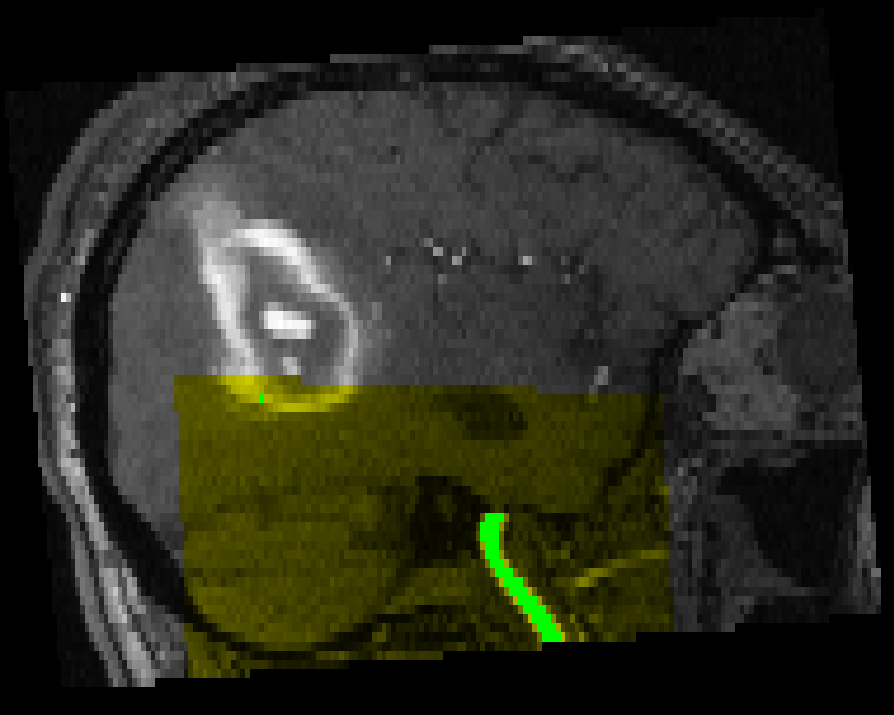
\includegraphics[width=\textwidth]{figures/molgu07704_bbox.png}
		\caption{}
		\label{subfig:seg_bbox}
	\end{subfigure}
	\begin{subfigure}{0.45\textwidth}
		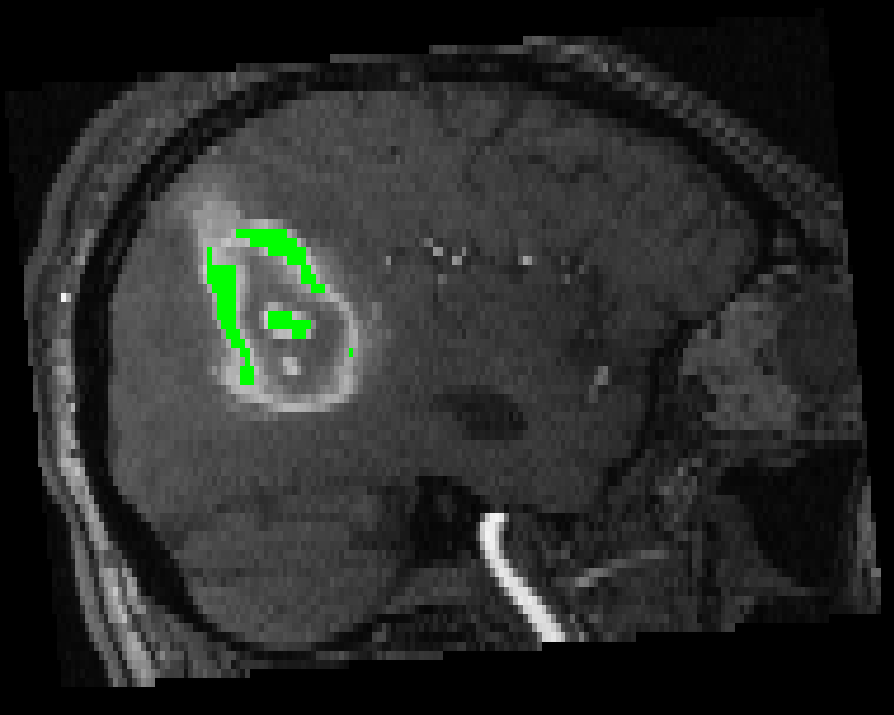
\includegraphics[width=\textwidth]{figures/molgu07704_nobbox.png}
		\caption{}
		\label{subfig:seg_nobbox}
	\end{subfigure}
	\caption{Comparison of carotid segmentation (green) with (a) and without (b) a cuboid mask (yellow). In the absence of the cuboid mask, the segmentation algorithm fails to capture the carotid and instead incorrectly identifies the brain lesion}
	\label{fig:seg_compare}
\end{figure}

\section{Hyperparameter Tuning}

The number of principle components $p$ was chosen as 3 by analysing the explained variance ratio plot in Figure~\ref{TODO}.
We see with only 3 components we get more than 90\% explained variability.
To prove the availability of the method, we seek to find the lowest possible number of population needed for the PCA in our \fdg $\,$ dataset.
To do this, the experiment was repeated 10 times each time with a different random seed for choosing population for $N=\{5,10,20,30,40,60\}$ and the resulting quantification errors were averaged.
As apparent in Figure~\ref{TODO}, we see a plateau in the performance after $N=10$ [TODO] and it was chosen as the ideal population sample count.

In model fitting using SA, an appropriate spectral range is chosen based on the radioisotope half-life (e.g. $10^{-4} \mathrm{s}^{-1}$ to $1 \mathrm{s}^{-1}$ for $^{18}\mathrm{F}$ ) and is then divided in to $s=100$ or $s=1000$ fixed frequencies ($\beta$) then their amplitudes ($\alpha$) are fitted to the TAC \ref{TODO}.
However, estimating 100 or 1000 different amplitude parameters using MCMC would not be computationally feasible.
Instead we must chose an appropriate number of spectral peaks and let the model to tune the frequencies and the amplitudes together.

To derive the number of basis functions, we assumed the activity in the surrounding tissue can either be modelled as 1TCM or 2TCM which their Impulse Response Function (IRF) have respectively one and two basis functions.
With two basis functions, it was found that the model rarely results in two distinctive frequencies and would generally converge to similar values.
Thus for both datasets one basis function was chosen.

As discussed in Section~\ref{TODO}, the prior distribution used for the PCA weighting coefficients was $\theta_i \sim \mathcal{N}(0,1)$.
The prior for the SA parameters were considered a very uninformative uniform distribution $\mathcal{U}(0,0.01)$ as we [TODO]


\section{Simulation}
From the 59 subjects in the \fdg $\,$ dataset, 24 subjects were excluded due to having very large brain tumors or opened skulls due to open brain surgery which caused the tissue classification algorithm to fail.
The rest of the 35 subjects were used to create the numerical phantoms




\section{IDIF}

Since BGTM relies on the GTM method and also depends on a population AIF. Thus the performance should be compared compared to the IDIF derived from GTM method and also the Population Based Input Function (PBIF) which is the mean AIF used in the PCA.


Figure~\ref{fig:ifs} compares the two methods for one of the best- and worst-performing subjects.
In the well-performing subject, BGTM significantly outperforms GTM ($\mrglu$ MAPE of 3.1\% vs. 20.9\%); however, in the poorly performing case, BGTM falls short of GTM ($\mrglu$ MAPE of 31.4\% vs. 19.5\%).
The average mean absolute error of the cAUC curves across the dataset was 14,202 for BGTM and 33,764 for GTM (Figure~\ref{subfig:cauc_boxplot}).

\begin{figure}[h]
	\centering
	\begin{subfigure}[b]{0.322\textwidth}
		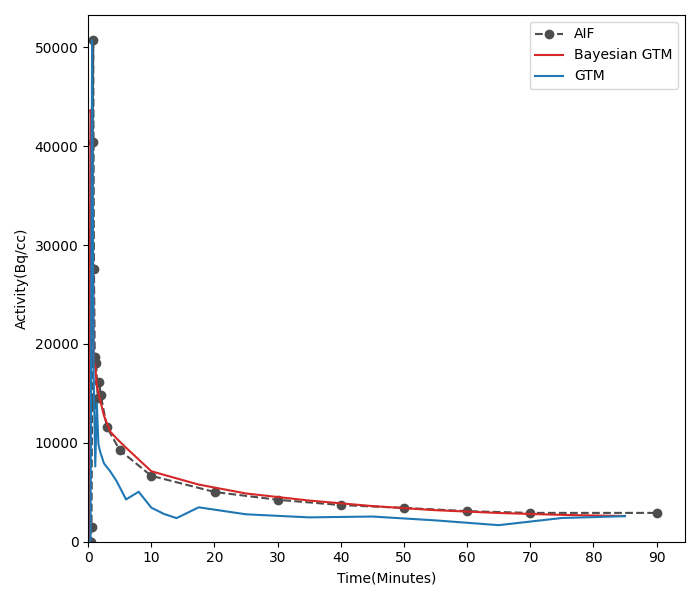
\includegraphics[width=\textwidth]{figures/MOLGU07704_1_if_comparison.png}
		\caption{}
		\label{subfig:good_if_compare}
	\end{subfigure}
	\begin{subfigure}[b]{0.322\textwidth}
		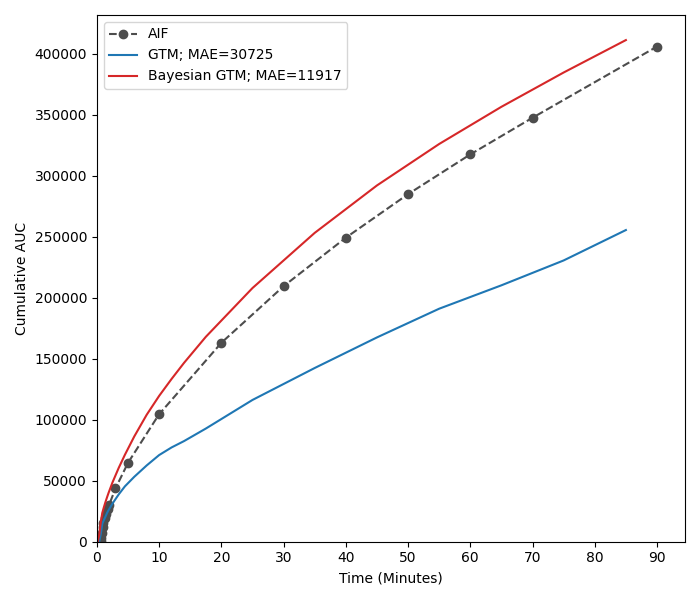
\includegraphics[width=\textwidth]{figures/MOLGU07704_1_trap.png}
		\caption{}
		\label{subfig:good_trap_compare}
	\end{subfigure}
	\begin{subfigure}[b]{0.322\textwidth}
		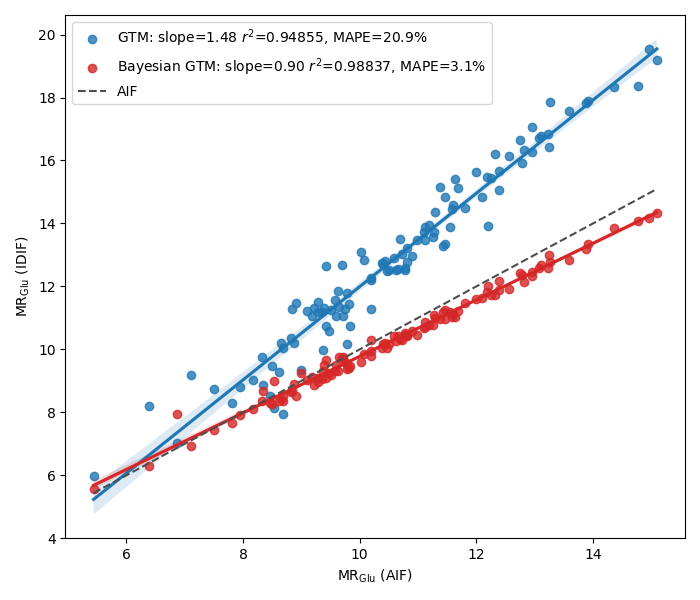
\includegraphics[width=\textwidth]{figures/MOLGU07704_1_cmrglu.png}
		\caption{}
		\label{fig:good_cmrglu}
	\end{subfigure}
	\begin{subfigure}[b]{0.322\textwidth}
		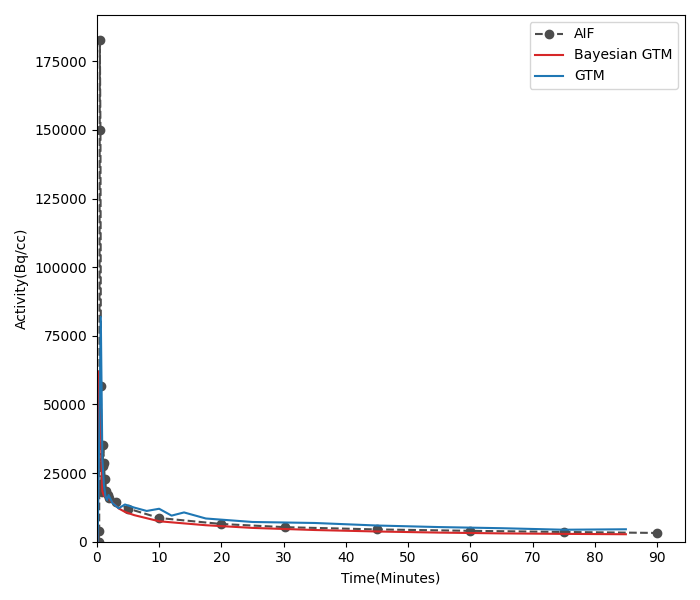
\includegraphics[width=\textwidth]{figures/CM10250_1_if_comparison.png}
		\caption{}
		\label{subfig:bad_if_compare}
	\end{subfigure}
	\begin{subfigure}[b]{0.322\textwidth}
		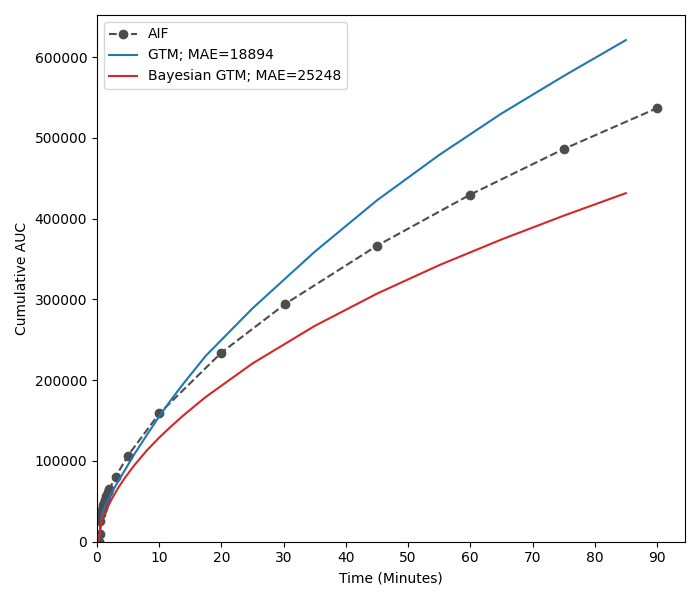
\includegraphics[width=\textwidth]{figures/CM10250_1_trap.png}
		\caption{}
		\label{subfig:bad_trap_compare}
	\end{subfigure}
	\begin{subfigure}[b]{0.322\textwidth}
		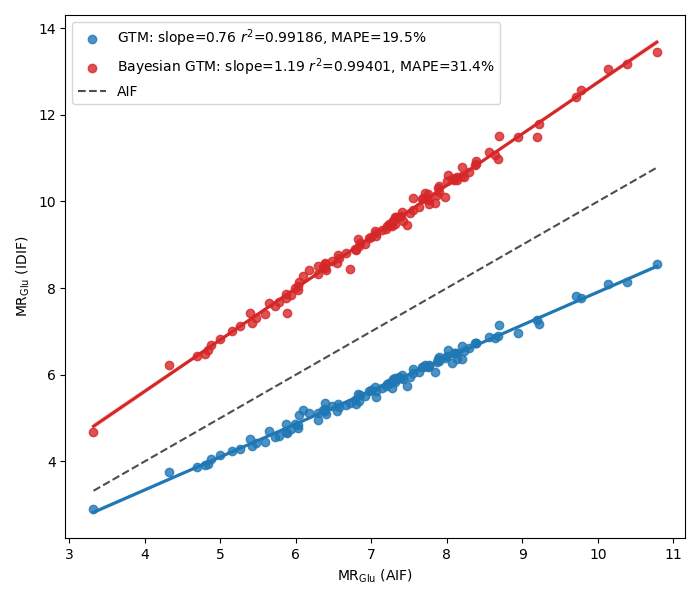
\includegraphics[width=\textwidth]{figures/CM10250_1_cmrglu.png}
		\caption{}
		\label{fig:bad_cmrglu}
	\end{subfigure}
	\caption{Comparison of the IFs (a,d), cumulative AUC curves (b,e), and $\mrglu$ regression lines (c,f) for one of the best-(top row) and worst-performingr(bottom row) subjects}
	\label{fig:ifs}
\end{figure}

ROI-based quantification was carried out using both IDIF methods, with BGTM yielding significantly better performance.
Specifically, the BGTM and GTM methods achieved an average \(\mrglu\) mean absolute percentage error (MAPE) of 14.1\% and 33\%, respectively (Figure~\ref{subfig:mape_boxplot}), and an average \(\mrglu\) MAE of 1.42 and 3.5.
In addition, the MAE for the coefficient of determination (\(R^2\)) and the regression slope (\(S\)) were 0.004 and 0.14 for BGTM, compared to 0.030 and 0.304 for GTM, respectively.

\begin{figure}
	\centering
	\begin{subfigure}[b]{0.45\textwidth}
		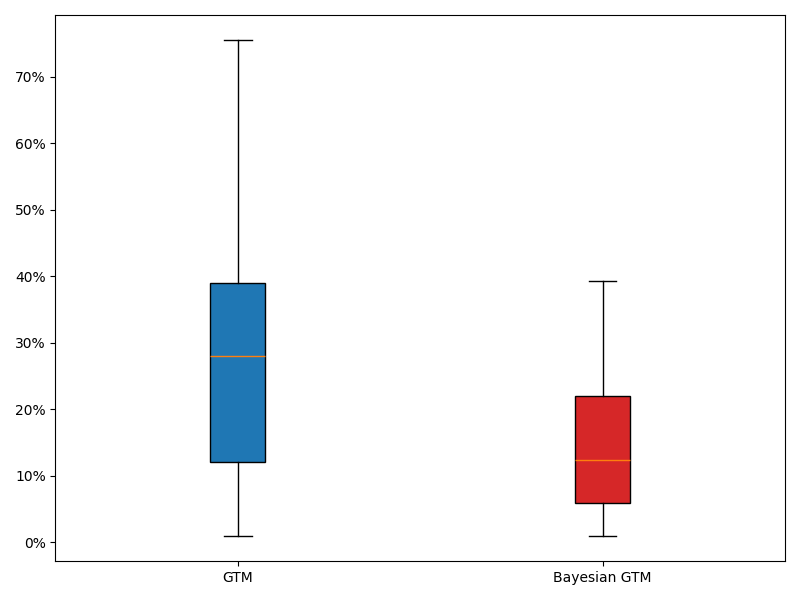
\includegraphics[width=\textwidth]{figures/quantification_mape_fitk3_boxplot.png}
		\caption{\(\mrglu\) MAPE Boxplot}
		\label{subfig:mape_boxplot}
	\end{subfigure}
	\begin{subfigure}[b]{0.45\textwidth}
		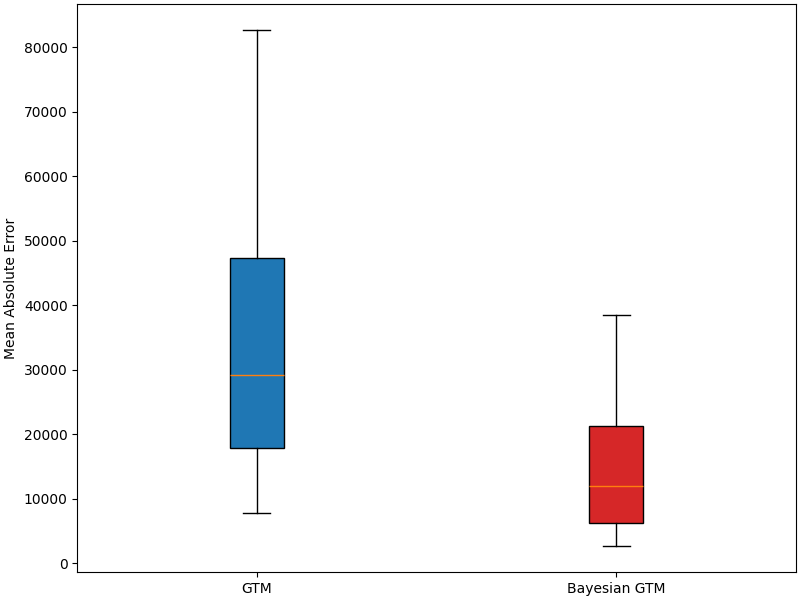
\includegraphics[width=\textwidth]{figures/curve_errors_boxplots.png}
		\caption{cAUC MAE Boxplot}
		\label{subfig:cauc_boxplot}
	\end{subfigure}
	\caption{Boxplot of curve and quantification errors}
	\label{fig:boxplots}
\end{figure}

\begin{table}[b]
	\centering
	\begin{tabular}{l|cc|cc|cc}
		\toprule
		\multirow{3}{*}{\textbf{Metric}} & \multicolumn{2}{c|}{\textbf{BGTM}} & \multicolumn{2}{c}{\textbf{GTM}} & \multicolumn{2}{c}{\textbf{Paired T-Test}}                                                 \\
		\cmidrule(lr){2-3} \cmidrule(lr){4-5} \cmidrule(lr){6-7}
		                                 & \(\mu\)                            & \(\sigma\)                       & \(\mu\)                                    & \(\sigma\) & T-Value & P-Value                \\
		\midrule
		IF cAUC MAE                      & 14,202                             & 9,190                            & 33,764                                     & 21,212     & 7.44    & \(7.2\times 10^{-10}\) \\
		$\mrglu$ MAPE (\%)               & 14.1                               & 10.1                             & 33.0                                       & 31.5       & 4.32    & \(6.5\times 10^{-5}\)  \\
		$\mrglu$ MAE                     & 1.42                               & 1.07                             & 3.50                                       & 3.38       & 4.41    & \(4.8\times 10^{-5}\)  \\
		$\mrglu$ \(R^2\) MAE             & 0.004                              & 0.006                            & 0.030                                      & 0.132      & 1.45    & \(1.5\times 10^{-1}\)  \\
		$\mrglu$ Slope MAE               & 0.14                               & 0.109                            & 0.304                                      & 0.230      & 4.73    & \(1.6\times 10^{-5}\)  \\
		\bottomrule
	\end{tabular}
	\caption{Summary of performance metrics for BGTM and GTM methods and their paired t-test.
		% $\mu$ is the average and $\sigma$ is the standard deviation
	}
	\label{tab:metrics}
\end{table}

A paired t-test was conducted to compare the performance of BGTM and GTM across previously mentioned metrics.
The results, summarized in Table~\ref{tab:metrics}, indicate that BGTM significantly outperforms GTM in cAUC MAE(\( t = 7.44 \), \( p = 7.2 \times 10^{-10} \)), $\mrglu$ MAPE (\( t = 4.32 \), \( p = 6.5 \times 10^{-5} \)), $\mrglu$ MAE (\( t = 4.41 \), \( p = 4.8 \times 10^{-5} \)), and $\mrglu$ Slope MAE (\( t = 4.73 \), \( p = 1.6 \times 10^{-5} \)), demonstrating the effectiveness of the proposed method.
However, no significant difference was observed in $\mrglu$ \(R^2\) MAE (\( t = 1.45 \), \( p = 0.15 \)).

As illustrated in Figure~\ref{fig:corr_mat}, there is a strong correlation between the cAUC MAE and the quantification errors suggesting cAUC as a reliable intermediate metric.

\begin{figure}[h]
	\centering
	\begin{subfigure}{0.45\textwidth}
		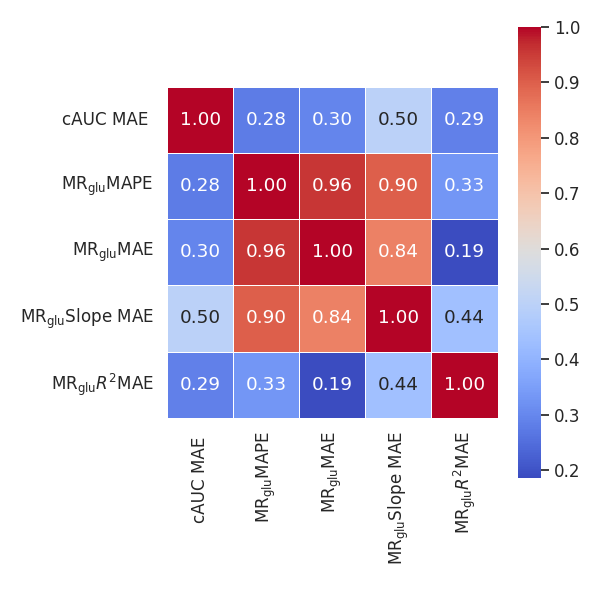
\includegraphics[width=\textwidth]{figures/corr_gtm.png}
		\caption{GTM}
		\label{subfig:corr_gtm}
	\end{subfigure}
	\begin{subfigure}{0.45\textwidth}
		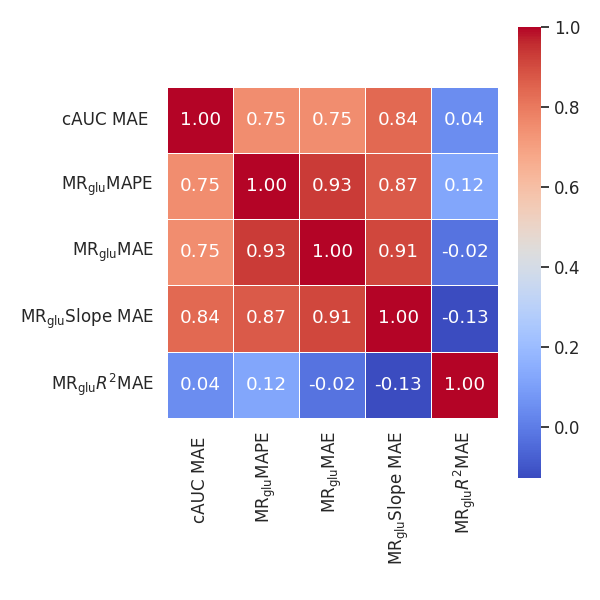
\includegraphics[width=\textwidth]{figures/corr_bgtm.png}
		\caption{Bayesian GTM}
		\label{subfig:corr_bgtm}
	\end{subfigure}
	\caption{Correlation matrix of different metrics for Bayesian GTM and GTM methods}
	\label{fig:corr_mat}
\end{figure}



